% Class Notes Template
\documentclass[12pt]{article}
\usepackage[margin=1in]{geometry}
\usepackage[utf8]{inputenc}

% Packages
\usepackage{amsmath, amsthm, amssymb ,amsfonts, graphics, tikz, float, enumerate}
\usepackage{listings,verbatim}
\usepackage{booktabs}
\usepackage{siunitx}
\usepackage{color} %red, green, blue, yellow, cyan, magenta, black, white
\definecolor{mygreen}{RGB}{28,172,0} % color values Red, Green, Blue
\definecolor{mylilas}{RGB}{170,55,241}

\lstset{language=Matlab,%
	%basicstyle=\color{red},
	breaklines=true,%
	morekeywords={matlab2tikz},
	keywordstyle=\color{blue},%
	morekeywords=[2]{1}, keywordstyle=[2]{\color{black}},
	identifierstyle=\color{black},%
	stringstyle=\color{mylilas},
	commentstyle=\color{mygreen},%
	showstringspaces=false,%without this there will be a symbol in the places where there is a space
	numbers=left,%
	numberstyle={\tiny \color{black}},% size of the numbers
	numbersep=9pt, % this defines how far the numbers are from the text
	emph=[1]{for,end,break},emphstyle=[1]\color{blue}, %some words to emphasise
	%emph=[2]{word1,word2}, emphstyle=[2]{style},
}

% Title
\title{ECON 7510 - BLP Replication}
\date{\today}
\author{Julien Manuel Neves}

% Use these for theorems, lemmas, proofs, etc.
\newtheorem{theorem}{Theorem}
\newtheorem{corollary}[theorem]{Corollary}
\newtheorem{lemma}[theorem]{Lemma}
\newtheorem{observation}[theorem]{Observation}
\newtheorem{proposition}[theorem]{Proposition}
\newtheorem{definition}[theorem]{Definition}
\newtheorem{claim}[theorem]{Claim}
\newtheorem{fact}[theorem]{Fact}
\newtheorem{assumption}[theorem]{Assumption}
\newtheorem{problem}[theorem]{Problem}
\newtheorem{set-up}[theorem]{Set-up}
\newtheorem{example}[theorem]{Example}
\newtheorem{remark}[theorem]{Remark}
\newtheorem{axiom}[theorem]{Axiom}

% Usefuls Macros
\newcommand{\field}[1]{\mathbb{#1}}
\newcommand{\N}{\field{N}} % natural numbers
\newcommand{\R}{\field{R}} % real numbers
\newcommand{\Z}{\field{Z}} % integers
\newcommand\F{\mathcal{F}}
\newcommand\B{\mathbb{B}}
\renewcommand{\Re}{\R} % reals
\newcommand{\Rn}[1]{\mathbb{R}^{#1}}
\newcommand{\1}{{\bf 1}} % vector of all 1's
\newcommand{\I}[1]{\mathbb{I}_{\left\{#1\right\}}} % indicator function
\newcommand{\La}{\mathscr{L}}
% \newcommand{\tends}{{\rightarrow}} % arrow for limits
% \newcommand{\ra}{{\rightarrow}} % abbreviation for right arrow
% \newcommand{\subjectto}{\mbox{\rm subject to}} % subject to

%% math operators
\DeclareMathOperator*{\argmin}{arg\,min}
\DeclareMathOperator*{\argmax}{arg\,max}
\DeclareMathOperator*{\maximize}{maximize}
\DeclareMathOperator*{\minimize}{minimize}
\DeclareMathOperator{\E}{\mathbb{E}} % expectation
\newcommand{\Ex}[1]{\E\left\{#1\right\}} % expectation with brackets
\DeclareMathOperator{\pr}{\mathsf{P}} % probability
\newcommand{\prob}[1]{\pr\left\{#1\right\}}
\DeclareMathOperator{\subjectto}{{s.t.\ }} % subject to
\newcommand{\norm}[1]{\left\|#1\right\|}
\newcommand{\card}[1]{\left|#1\right|}

% Extra stuff
\newcommand\seq[1]{\{ #1 \}}
\newcommand{\inp}[2]{\langle #1, #2 \rangle}

\newcommand{\inv}{^{-1}}

\newcommand{\pa}[1]{\left(#1\right)}
\newcommand{\bra}[1]{\left[#1\right]}
\newcommand{\cbra}[1]{\left\{ #1 \right\}}

\newcommand{\pfrac}[2]{\pa{\frac{#1}{#2}}}
\newcommand{\bfrac}[2]{\bra{\frac{#1}{#2}}}

\newcommand{\mat}[1]{\begin{matrix}#1\end{matrix}}
\newcommand{\pmat}[1]{\pa{\mat{#1}}}
\newcommand{\bmat}[1]{\bra{\mat{#1}}}

\begin{document}

\maketitle

\section*{Part 1}

From the problem set description, we start by assuming that each consumer $i$
has utility for product $j$ as a function of price and product quality, $\delta_j$ of:
\[
u_{ij} =\delta_j -\alpha_i p_j
\]
The distribution of consumer price sensitivity, $\alpha_i$, is exponential with parameter $\lambda = 4\cdot 10^{-6}$. We further assume that $\delta_j = x_j\beta +\xi_j$ and that $x_j$ is uncorrelated with $\xi_j$.

In this model, $i$ choose the $j$ that provides the highest utility. This implies that if $p_j>p_k$, we need $\delta_j>\delta_k$ otherwise no one would ever pick $j$. In the same vein, it is straightforward to see that the share of good $j$ will depend only on its close neighbors in the price dimension. Hence, before deriving the result, we sort the data from lowest to highest price.

As mentionned above, to determine $j$ share we only need to compare its $u_{ij}$ to $j-1$ and $j+1$. In fact, $i$ will choose $j$ if and only if
\[
u_{i,j}>u_{i,j-1} \text{ and } u_{i,j}>u_{i,j+1}
\]

This boils down to the following condition for $\alpha_i$
\[
\frac{\delta_{j+1}-\delta_{j}}{p_{j+1}-p_{j}}<\alpha_i<\frac{\delta_j-\delta_{j-1}}{p_j-p_{j-1}}
\]
and therefore the share of good $j$ is given by
\begin{align*}
	s_j&=\int_{\frac{\delta_{j+1}-\delta_{j}}{p_{j+1}-p_{j}}}^{\frac{\delta_j-\delta_{j-1}}{p_j-p_{j-1}}}f(x)dx\\
	& = F\left({\frac{\delta_j-\delta_{j-1}}{p_j-p_{j-1}}}\right) - F\left( {\frac{\delta_{j+1}-\delta_{j}}{p_{j+1}-p_{j}}}\right)
\end{align*}
where $F(x)= 1-e^{-\lambda x}$.

Since we know $s_j$ and $p_j$, we can recursively solve for $\delta_j$, by noting that the following relationship holds
\[
\ln\left(\sum_{k=0}^j s_k\right) = -\lambda \left({\frac{\delta_{j+1}-\delta_{j}}{p_{j+1}-p_{j}}}\right)
\]

Using our $\delta_j$, we can compute our estimate for $\beta$ with simple OLS since we assume that $\Ex{x_j\xi_j}=0$. The results are stated in Table \ref{tab:vertical}.

\begin{table}[H]\centering
\caption{Vertical model - Demand side only}
\begin{tabular}{c c }
\toprule
 & \textbf{Demand side} \\
\midrule
(Intercept)         &     \num{7.5865 e+7} \\
    &      [\num{3.9391 e+7}  \num{1.1234 e+8}]      \\
Weight         &     \num{4.1722 e+4} \\
  &      [\num{2.5642 e+4}  \num{5.7802 e+4}]      \\
Horsepower         &     \num{3.1989 e+5} \\
      &      [\num{1.2081 e+5}  \num{5.1897 e+5}]      \\
AC         &     \num{1.1753 e+7} \\
	     &      [\num{-4.3171 e+6}  \num{2.7823 e+7}]      \\
FE       &      Yes \\
            &     \\
\midrule
 N           &     131     \\
R$^{2}$           &       0.8175   \\
\bottomrule
\addlinespace[1ex]
$[\quad] $ 95\% confidence interval
\end{tabular}
 \label{tab:vertical}
\end{table}

Note that while the regression in Table \ref{tab:vertical} includes fixed effects for the firm, I simply don't report their values for the sake of conciseness.


\section*{Part 2}

Note that if two goods, for example $j$ and $k$, have the same price and strictly positive shares in this model we need that $\delta_k=\delta_j$ and hence $u_{ik}=u_{ij}$ for all consumer. If not, one good would have zero market share. This is a fairly extreme assumption.

Looking at Table \ref{tab:vertical_elasticities}, we can see that the model insinuates rather odd own and cross price elasticities.
\begin{table}[H]
	\centering
	\caption{Vertical model - Price elasticities}
	\resizebox{\columnwidth}{!}{%
\begin{tabular}{lllllllllll}
	\toprule
Car$\backslash$Car & 15      & 16      & 17                                & 18      & 19      &
20      & 21      & 22      & 23      & 24      \\
\midrule
15                     & -0.0948 & 0.0003  & 0                                 & 0       & 0       & 0       & 0       & 0       & 0       & 0       \\
16                     & 0.0003  & -0.0003 & 0.0000 & 0       & 0       & 0       & 0       & 0       & 0       & 0       \\
17                     & 0       & 0.0001  & -0.0671                           & 0.0673  & 0       & 0       & 0       & 0       & 0       & 0       \\
18                     & 0       & 0       & 0.0050                            & -0.0154 & 0.0104  & 0       & 0       & 0       & 0       & 0       \\
19                     & 0       & 0       & 0                                 & 0.0711  & -0.5703 & 0.4997  & 0       & 0       & 0       & 0       \\
20                     & 0       & 0       & 0                                 & 0       & 0.1349  & -0.1477 & 0.0126  & 0       & 0       & 0       \\
21                     & 0       & 0       & 0                                 & 0       & 0       & 0.0235  & -0.0438 & 0.0202  & 0       & 0       \\
22                     & 0       & 0       & 0                                 & 0       & 0       & 0       & 1.2703  & -1.8608 & 0.5881  & 0       \\
23                     & 0       & 0       & 0                                 & 0       & 0       & 0       & 0       & 0.0175  & -0.0180 & 0.0004  \\
24                     & 0       & 0       & 0                                 & 0       & 0       & 0       & 0       & 0       & 0.0001  & -0.0390\\
\bottomrule
\end{tabular}%
}
 \label{tab:vertical_elasticities}
\end{table}

This weird pattern stems from the fact that cross price elasticities for any given good is going to be equal to zero apart from its direct neighbors. It is straightforward to show this fact by noting that $s_j= F\left({\frac{\delta_j-\delta_{j-1}}{p_j-p_{j-1}}}\right) - F\left( {\frac{\delta_{j+1}-\delta_{j}}{p_{j+1}-p_{j}}}\right)$ is not a function of any price but $p_j$, $p_{j-1}$, and $p_{j+1}$.

\section*{Part 3}

We know turn our attention to the supply side of our model. We are given the following equation for marginal cost $mc_j = x_j\gamma +\eta q_j +\omega_j$. Sadly we don't have the actual value for the marginal cost. We can circumvent this issue by relating marginal cost to price by assuming some pricing strategy for the firms. As a matter of fact, these pricing strategy will result in a markup over marginal cost given by the following formulas:
\begin{itemize}
	\item Marginal cost pricing:
	\[
p_j = mc_j
	\]
	\item Single product firms:
	\[
p_j = mc_j +\Delta\inv s
	\]
	where $\Delta_{jk} = \left\{\mat{\frac{\partial s_j}{\partial p_k} & \text{if }j=k\\ 0 & \text{otherwise}}\right.$ and $s$ is the vector of shares.

	\item Multiproduct firms:
	\[
p_j = mc_j +\Delta\inv s
	\]
	where $\Delta_{jk} = \left\{\mat{\frac{\partial s_j}{\partial p_k} & \text{if }k\in \text{firm}(j)\\ 0 & \text{otherwise}}\right.$ and $s$ is the vector of shares.

	\item Perfect collusion:
	\[
p_j = mc_j +\Delta\inv s
	\]
	where $\Delta_{jk} = \frac{\partial s_j}{\partial p_k} $ and $s$ is the vector of shares.
\end{itemize}

From the previous question, it is easy to to compute $\Delta$ and therefore $mc_j$.

With this in mind we can revert back to $mc_j = x_j\gamma +\eta q_j +\omega_j$ and estimate it like we would for $\delta_j = x_j\beta +\xi_j$. The only issue we are facing now is	the potential endogeneity of $q_j$.

To remedy the situation, we need to find an instrument for $q_j$. There is plenty potential instruments, but after playing around for a while, I decide to follow Gandhi and Houde (2018) and use $\sum_k |x_j-x_k|$ and $\sum_k (x_j - x_k)^2$. To avoid any problem with collinearity and matrix inversion, I use the function \verb!licols()! to reduce our set of instruments $Z = [x_j,\sum_k |x_j - x_k|, \sum_k (x_j - x_k)^2]$ to a full column rank matrix.

The result from our IV regression, using the different pricing strategy, are given in Table \ref{tab:tab:vertical_supply}.


\begin{table}[H]\centering
\caption{Vertical model - supply side}
\resizebox{\columnwidth}{!}{%
\begin{tabular}{c c c c c}
\toprule
 & \textbf{Marginal cost} & \textbf{Single product firms} & \textbf{Multiproduct firms} & \textbf{Collusion} \\
\midrule
(Intercept)         &     \num{7.5865 e+7}  &     \num{7.5865 e+7} &     \num{7.5865 e+7} &     \num{7.5865 e+7} \\
    &      [\num{3.9391 e+7}  \num{1.1234 e+8}]       &      [\num{3.9391 e+7}  \num{1.1234 e+8}]     &      [\num{3.9391 e+7}  \num{1.1234 e+8}]     &      [\num{3.9391 e+7}  \num{1.1234 e+8}]    \\
Weight         &     \num{4.1722 e+4}    &     \num{4.1722 e+4}    &     \num{4.1722 e+4}    &     \num{4.1722 e+4} \\
  &      [\num{2.5642 e+4}  \num{5.7802 e+4}] &      [\num{2.5642 e+4}  \num{5.7802 e+4}]  &      [\num{2.5642 e+4}  \num{5.7802 e+4}]  &      [\num{2.5642 e+4}  \num{5.7802 e+4}]       \\
Horsepower         &     \num{3.1989 e+5}  &     \num{3.1989 e+5} &     \num{3.1989 e+5} &     \num{3.1989 e+5}\\
      &      [\num{1.2081 e+5}  \num{5.1897 e+5}]  &      [\num{1.2081 e+5}  \num{5.1897 e+5}]&      [\num{1.2081 e+5}  \num{5.1897 e+5}]&      [\num{1.2081 e+5}  \num{5.1897 e+5}]    \\
AC         &     \num{1.1753 e+7}    &     \num{1.1753 e+7}   &     \num{1.1753 e+7}   &     \num{1.1753 e+7}\\
	     &      [\num{-4.3171 e+6}  \num{2.7823 e+7}]   &      [\num{-4.3171 e+6}  \num{2.7823 e+7}]  &      [\num{-4.3171 e+6}  \num{2.7823 e+7}]  &      [\num{-4.3171 e+6}  \num{2.7823 e+7}]     \\
FE       &      Yes & Yes & Yes & Yes \\
            &     \\
\midrule
 N           &     131 &     131 &     131 &     131     \\
R$^{2}$           &       0.8175  &       0.8175 &       0.8175 &       0.8175  \\
	\midrule
	(Intercept)         &     \num{7.5865 e+7}  &     \num{7.5865 e+7} &     \num{7.5865 e+7} &     \num{7.5865 e+7} \\
 &      [\num{3.9391 e+7}  \num{1.1234 e+8}]       &      [\num{3.9391 e+7}  \num{1.1234 e+8}]     &      [\num{3.9391 e+7}  \num{1.1234 e+8}]     &      [\num{3.9391 e+7}  \num{1.1234 e+8}]    \\
		Weight         &     \num{4.1722 e+4}    &     \num{4.1722 e+4}    &     \num{4.1722 e+4}    &     \num{4.1722 e+4} \\
 &      [\num{2.5642 e+4}  \num{5.7802 e+4}] &      [\num{2.5642 e+4}  \num{5.7802 e+4}]  &      [\num{2.5642 e+4}  \num{5.7802 e+4}]  &      [\num{2.5642 e+4}  \num{5.7802 e+4}]       \\
Horsepower         &     \num{3.1989 e+5}  &     \num{3.1989 e+5} &     \num{3.1989 e+5} &     \num{3.1989 e+5}\\
	      &      [\num{1.2081 e+5}  \num{5.1897 e+5}]  &      [\num{1.2081 e+5}  \num{5.1897 e+5}]&      [\num{1.2081 e+5}  \num{5.1897 e+5}]&      [\num{1.2081 e+5}  \num{5.1897 e+5}]    \\
	AC         &     \num{1.1753 e+7}    &     \num{1.1753 e+7}   &     \num{1.1753 e+7}   &     \num{1.1753 e+7}\\
		     &      [\num{-4.3171 e+6}  \num{2.7823 e+7}]   &      [\num{-4.3171 e+6}  \num{2.7823 e+7}]  &      [\num{-4.3171 e+6}  \num{2.7823 e+7}]  &      [\num{-4.3171 e+6}  \num{2.7823 e+7}]     \\
Quantity         &     \num{7.5865 e+7}  &     \num{7.5865 e+7} &     \num{7.5865 e+7} &     \num{7.5865 e+7} \\
 &      [\num{3.9391 e+7}  \num{1.1234 e+8}]       &      [\num{3.9391 e+7}  \num{1.1234 e+8}]     &      [\num{3.9391 e+7}  \num{1.1234 e+8}]     &      [\num{3.9391 e+7}  \num{1.1234 e+8}]    \\

	FE       &      Yes & Yes & Yes & Yes \\
						            &     \\
\midrule
 N           &     131 &     131 &     131 &     131     \\
R$^{2}$           &       0.8175   \\
\bottomrule
\addlinespace[1ex]
$[\quad] $ 95\% confidence interval
\end{tabular}%
}
 \label{tab:vertical_supply}
\end{table}

%%%%%%%%%%%
 %% Need to talk about results and change theorem
 %%%%%%%%%%%%
\section*{Part 4}
%%%%%%%%%%%
 %% Need to talk about how to test which supply
 %%%%%%%%%%%%

\section*{Part 5}

We now assume that each consumer $i$ has utility for product $j$ as a function of price and product quality, $\delta_j$ of:
\[
u_{ij} =\delta_j +\epsilon_{ij}
\]
where $\delta_j = x_j\beta -\alpha p_j+\xi_j$, $\xi_j$ is the unosbervable characteristics of good $j$ and $\epsilon_{ij}$ follows a type I extreme value distribution.

As shown in class, we have that the share of good $j$ is given by
\[
s_j = \frac{e^{\delta_j }}{1+\sum_k e^{\delta_k}}
\]
or, equivalently,
\[
\ln(s_j)-\ln(s_0) = x_j\beta -\alpha p_j+\xi_j
\]

Armed with this regression, we can now estimate $[\beta, \alpha]$. Like with the supply side, we now have some endogeneity problem. To solve this, we use the same set of instruments, $Z = [x_j,\sum_k |x_j - x_k|, \sum_k (x_j - x_k)^2]$, and run an IV regression to get back both $[\beta, \alpha]$ and $\xi$. The result from our IV regression are reported in Table \ref{tab:logit}.

Moreover, Table  \ref{tab:logit} includes the estimation of demand and supply parameters assuming Nash-Bertrand equilibrium with multiproduct firms. Recall that with multiproduct firms, Nash-Bertrand equilibrium yields
\[
p = mc + \Delta\inv s  = \Delta\inv s + x\gamma +\eta q +\omega
\]
where $\Delta_{jk} = \left\{\mat{\frac{\partial s_j}{\partial p_k} & \text{if }k\in \text{firm}(j)\\ 0 & \text{otherwise}}\right.$ and $s$ is the vector of shares. We can solve explicitly for $\Delta$ by noting that $\frac{\partial s_j}{\partial p_k}= \left\{\mat{ -\alpha s_j(1-s_j) & \text{if } j= k\\ \alpha s_js_k & \text{otherwise}}\right.$. Let $\Delta\inv s = b(\alpha)$ since, unlike the vertical model, it depends on $\alpha$ in a non-linear fashion.

We can now define our moments equations:
\begin{align*}
	\Ex{\mat{Z\xi_j \\ Z\omega_j}} = 0
\end{align*}
or, equivalently
\begin{align*}
	\Ex{\mat{Z(\delta_j - x_j\beta +\alpha p_j) \\ Z(p_j-b_j(\alpha)-x_j\gamma -\eta q_j)}} = 0
\end{align*}
where $Z$ is the set of instruments. Using these statcked moments conditions, we can use our usual GMM technique to estimate $\theta = [\alpha, \beta, \gamma, \eta]$. Since $\alpha$ enters non-linearly, to solve for it I use \verb!fmincon()! to minize the objective function with respect to $\alpha$ and then solve for the rest of parameters using least squares techniques.

The only issue that I'm facing now is how to compute the standard errors of our estimate. Since, $\alpha$ enters non-linearly, I need to find the gradient of $s_j$ with $\theta$ to be able to compute the GMM covariance matrix. Sadly, I ran out of time. Estimation results are reported in Table \ref{tab:logit}.

\begin{table}[H]\centering
\caption{Vertical model - supply side}
\resizebox{\columnwidth}{!}{%
\begin{tabular}{c c c}
\toprule
 & \textbf{Marginal cost} & \textbf{Multiple product firms} \\
\midrule
(Intercept)         &     \num{7.5865 e+7}  &     \num{7.5865 e+7}  \\
    &      [\num{3.9391 e+7}  \num{1.1234 e+8}]       &             \\
Weight         &     \num{4.1722 e+4}    &     \num{4.1722 e+4}     \\
  &      [\num{2.5642 e+4}  \num{5.7802 e+4}] &           \\
Horsepower         &     \num{3.1989 e+5}  &     \num{3.1989 e+5} \\
      &      [\num{1.2081 e+5}  \num{5.1897 e+5}]  &      \\
AC         &     \num{1.1753 e+7}    &     \num{1.1753 e+7}  \\
	     &      [\num{-4.3171 e+6}  \num{2.7823 e+7}]   &         \\
Price ($\alpha$)         &     \num{1.1753 e+7}    &     \num{1.1753 e+7}  \\
			 	     &      [\num{-4.3171 e+6}  \num{2.7823 e+7}]   &           \\
FE       &      Yes & Yes \\
            &     \\
\midrule
 N           &     131 &     131      \\
R$^{2}$           &       0.8175   \\
	\midrule
	(Intercept)         &       &     \num{7.5865 e+7} \\
 &            &           \\
		Weight         &       &     \num{4.1722 e+4}     \\
 &      &       \\
Horsepower         &       &     \num{3.1989 e+5} \\
	      &       &       \\
	AC         &        &     \num{1.1753 e+7} \\
		     &         &        \\
Quantity         &      &     \num{7.5865 e+7}  \\
 &             &          \\

	FE       &   & Yes  \\
						            &     \\
\midrule
 N           &     131 &     131      \\
R$^{2}$           &       0.8175   \\
\bottomrule
\addlinespace[1ex]
$[\quad] $ 95\% confidence interval
\end{tabular}%
}
 \label{tab:logit}
\end{table}

Again, we report the elasticities for a subset of the product in Table \ref{tab:logit_elasticities}.

\begin{table}[H]
	\centering
	\caption{Vertical model - Price elasticities}
	\resizebox{\columnwidth}{!}{%
\begin{tabular}{lllllllllll}
	\toprule
Car$\backslash$Car & 15      & 16      & 17                                & 18      & 19      &
20      & 21      & 22      & 23      & 24      \\
\midrule
15                     & -0.0948 & 0.0003  & 0                                 & 0       & 0       & 0       & 0       & 0       & 0       & 0       \\
16                     & 0.0003  & -0.0003 & 0.0000 & 0       & 0       & 0       & 0       & 0       & 0       & 0       \\
17                     & 0       & 0.0001  & -0.0671                           & 0.0673  & 0       & 0       & 0       & 0       & 0       & 0       \\
18                     & 0       & 0       & 0.0050                            & -0.0154 & 0.0104  & 0       & 0       & 0       & 0       & 0       \\
19                     & 0       & 0       & 0                                 & 0.0711  & -0.5703 & 0.4997  & 0       & 0       & 0       & 0       \\
20                     & 0       & 0       & 0                                 & 0       & 0.1349  & -0.1477 & 0.0126  & 0       & 0       & 0       \\
21                     & 0       & 0       & 0                                 & 0       & 0       & 0.0235  & -0.0438 & 0.0202  & 0       & 0       \\
22                     & 0       & 0       & 0                                 & 0       & 0       & 0       & 1.2703  & -1.8608 & 0.5881  & 0       \\
23                     & 0       & 0       & 0                                 & 0       & 0       & 0       & 0       & 0.0175  & -0.0180 & 0.0004  \\
24                     & 0       & 0       & 0                                 & 0       & 0       & 0       & 0       & 0       & 0.0001  & -0.0390\\
\bottomrule
\end{tabular}%
}
 \label{tab:logit_elasticities}
\end{table}

Looking at these elasticities, we have an improvment compared to the previous vertical model where most elasticities where equal to 0.


\section*{Part 6}
\section*{Part 7}
\section*{Part 8}


\begin{table}[H]\centering
\caption{Vertical model - Demand side only}
\begin{tabular}{c c }
\toprule
 & \textbf{Demand side} \\
\midrule
(Intercept)         &     \num{7.5865 e+7} \\
    &         \\
Weight         &     \num{4.1722 e+4} \\
  &          \\
Horsepower         &     \num{3.1989 e+5} \\
      &           \\
AC         &     \num{1.1753 e+7} \\
	     &           \\
Price ($\alpha_1$ )        &     \num{1.1753 e+7} \\
			 	     &         \\

Price ($\alpha_2$)         &     \num{1.1753 e+7} \\
  &            \\
						 \midrule
	FE       &      Yes \\
					 &     \\
\midrule
 N           &     131     \\
R$^{2}$           &       0.8175   \\
\bottomrule
\addlinespace[1ex]
$[\quad] $ 95\% confidence interval
\end{tabular}
 \label{tab:blp}
\end{table}


\begin{figure}
	\centering
	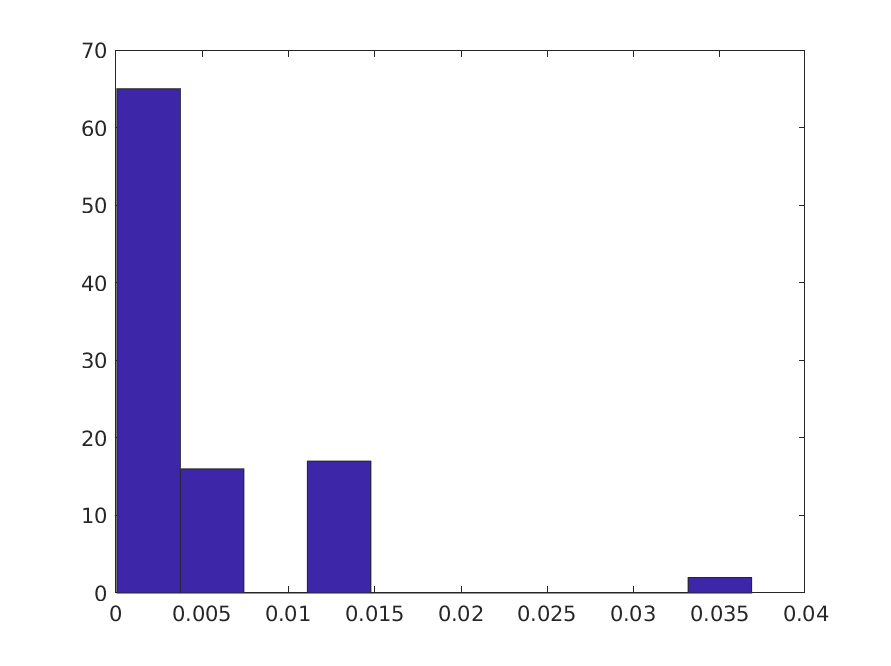
\includegraphics[width=0.7\linewidth]{../output/alpha2}
	\caption{}
	\label{fig:alpha2}
\end{figure}

\begin{table}[H]
	\centering
	\caption{Vertical model - Price elasticities}
	\resizebox{\columnwidth}{!}{%
\begin{tabular}{lllllllllll}
	\toprule
Car$\backslash$Price & 15      & 16      & 17                                & 18      & 19      &
20      & 21      & 22      & 23      & 24      \\
\midrule
15                     & -0.0948 & 0.0003  & 0                                 & 0       & 0       & 0       & 0       & 0       & 0       & 0       \\
16                     & 0.0003  & -0.0003 & 0.0000 & 0       & 0       & 0       & 0       & 0       & 0       & 0       \\
17                     & 0       & 0.0001  & -0.0671                           & 0.0673  & 0       & 0       & 0       & 0       & 0       & 0       \\
18                     & 0       & 0       & 0.0050                            & -0.0154 & 0.0104  & 0       & 0       & 0       & 0       & 0       \\
19                     & 0       & 0       & 0                                 & 0.0711  & -0.5703 & 0.4997  & 0       & 0       & 0       & 0       \\
20                     & 0       & 0       & 0                                 & 0       & 0.1349  & -0.1477 & 0.0126  & 0       & 0       & 0       \\
21                     & 0       & 0       & 0                                 & 0       & 0       & 0.0235  & -0.0438 & 0.0202  & 0       & 0       \\
22                     & 0       & 0       & 0                                 & 0       & 0       & 0       & 1.2703  & -1.8608 & 0.5881  & 0       \\
23                     & 0       & 0       & 0                                 & 0       & 0       & 0       & 0       & 0.0175  & -0.0180 & 0.0004  \\
24                     & 0       & 0       & 0                                 & 0       & 0       & 0       & 0       & 0       & 0.0001  & -0.0390\\
\bottomrule
\end{tabular}%
}
 \label{tab:blp_elasticities}
\end{table}

\section*{Part 9}

\section*{Code}
\subsection*{Problem 2}
%\lstinputlisting[language=Matlab]{../code/run_me}
%\lstinputlisting[language=Matlab]{../code/blp_model}
%\lstinputlisting[language=Matlab]{../code/create_IV}
%\lstinputlisting[language=Matlab]{../code/get_markup}
%\lstinputlisting[language=Matlab]{../code/get_mean_utility}
%\lstinputlisting[language=Matlab]{../code/get_shares}
%\lstinputlisting[language=Matlab]{../code/gmm_fun}
%\lstinputlisting[language=Matlab]{../code/logit_model}
%\lstinputlisting[language=Matlab]{../code/vertical_model}
%\lstinputlisting[language=Matlab]{../code/prepare_data}


\end{document}
